%definira klasu dokumenta 
\documentclass[12pt]{report} 

%prostor izmedu naredbi \documentclass i \begin{document} se zove uvod. U njemu se nalaze naredbe koje se odnose na cijeli dokument
	
	%osnovni LaTex ne može riješiti sve probleme, pa se koriste različiti paketi koji olakšavaju izradu željenog dokumenta
	\usepackage[croatian]{babel} 
	\usepackage{amssymb}
	\usepackage{amsmath}
	\usepackage{txfonts}
	\usepackage{mathdots}
	\usepackage{titlesec}
	\usepackage{array}
	\usepackage{lastpage}
	\usepackage{etoolbox}
	\usepackage{tabularray}
	\usepackage{color, colortbl}
	\usepackage{adjustbox}
	\usepackage{geometry}
	\usepackage[classicReIm]{kpfonts}
	\usepackage{hyperref}
	\usepackage{fancyhdr}
	\usepackage{placeins}
	
	\usepackage{float}
	\usepackage{setspace}
	\restylefloat{table}
	
	
	\patchcmd{\chapter}{\thispagestyle{plain}}{\thispagestyle{fancy}}{}{} %redefiniranje stila stranice u paketu fancyhdr
	
	%oblik naslova poglavlja
	\titleformat{\chapter}{\normalfont\huge\bfseries}{\thechapter.}{20pt}{\Huge}
	\titlespacing{\chapter}{0pt}{0pt}{40pt}
	
	
	\linespread{1.3} %razmak između redaka
	
	\geometry{a4paper, left=1in, top=1in,}  %oblik stranice
	
	\hypersetup{ colorlinks, citecolor=black, filecolor=black, linkcolor=black,	urlcolor=black }   %izgled poveznice
	
	
	%prored smanjen između redaka u nabrajanjima i popisima
	\newenvironment{packed_enum}{
		\begin{enumerate}
			\setlength{\itemsep}{0pt}
			\setlength{\parskip}{0pt}
			\setlength{\parsep}{0pt}
		}{\end{enumerate}}
	
	\newenvironment{packed_item}{
		\begin{itemize}
			\setlength{\itemsep}{0pt}
			\setlength{\parskip}{0pt}
			\setlength{\parsep}{0pt}
		}{\end{itemize}}
	
	
	
	
	%boja za privatni i udaljeni kljuc u tablicama
	\definecolor{LightBlue}{rgb}{0.9,0.9,1}
	\definecolor{LightGreen}{rgb}{0.9,1,0.9}
	
	%Promjena teksta za dugačke tablice
	\DefTblrTemplate{contfoot-text}{normal}{Nastavljeno na idućoj stranici}
	\SetTblrTemplate{contfoot-text}{normal}
	\DefTblrTemplate{conthead-text}{normal}{(Nastavljeno)}
	\SetTblrTemplate{conthead-text}{normal}
	\DefTblrTemplate{middlehead,lasthead}{normal}{Nastavljeno od prethodne stranice}
	\SetTblrTemplate{middlehead,lasthead}{normal}
	
	%podesavanje zaglavlja i podnožja
	
	\pagestyle{fancy}
	\lhead{Programsko inženjerstvo}
	\rhead{SpotPicker}
	\lfoot{Leteći medvjedići}
	\cfoot{stranica \thepage/\pageref{LastPage}}
	\rfoot{\today}
	\renewcommand{\headrulewidth}{0.2pt}
	\renewcommand{\footrulewidth}{0.2pt}
	
	
	\begin{document} 
		
		
		
		\begin{titlepage}
			\begin{center}
				\vspace*{\stretch{1.0}} %u kombinaciji s ostalim \vspace naredbama definira razmak između redaka teksta
				\LARGE Programsko inženjerstvo\\
				\large Ak. god. 2023./2024.\\
				
				\vspace*{\stretch{3.0}}
				
				\huge SpotPicker\\
				\Large Dokumentacija, Rev. 2  \\
				
				\vspace*{\stretch{12.0}}
				\normalsize
				Grupa: Leteći medvjedići\\
				Voditelj: Mario Olčar\\
				
				
				\vspace*{\stretch{1.0}}
				Datum predaje: 17. 11. 2023.\\
				
				\vspace*{\stretch{4.0}}
				
				Nastavnik: Hrvoje Nuić, mag. ing.\\
				
			\end{center}
			
			
		\end{titlepage}
		
		
		\tableofcontents
		
		\chapter{Dnevnik promjena dokumentacije}



\begin{longtblr}[
	label=none,
	entry=none
	]{
		width = \textwidth,
		colspec={|X[4,l]|X[8, l]|X[4, l]|X[4, l]|},
		rowhead = 1,
	} %definicija širine tablice, širine stupaca, poravnanje i broja redaka naslova tablice
	\hline
	\textbf{Rev.} & \textbf{Opis promjene/dodatka}	&  	\textbf{Autori}  & \textbf{Datum}	\\ \hline
	0.01 & Napravljen predložak & Mario Olčar  & 22.10.2023 \\ \hline
	0.10 & Dodan opis zadatka & Mario Olčar & 29.10.2023 \\ \hline
	0.19 & Dodani opisi obrazaca uporabe & Paula Močinić & 8.11.2023 \\ \hline
	0.28 & Dodani dijagrami obrazaca uporabe & Paula Močinić  & 8.11.2023 \\ \hline

	0.37 & Dodani sekvencijski dijagrami i njihovi opisi & Paula Močinić  & 9.11.2023 \\ \hline
	0.46 & Stvorena mapa sa slikama dijagrama & Paula Močinić  & 12.11.2023 \\ \hline
	0.55 & Dodani ostali zahtjevi & Paula Močinić  & 13.11.2023 \\ \hline
	0.61 & Dodani funkcijski zahtjevi & Ivan Bušljeta  & 15.11.2023 \\ \hline

	0.70 & Dodan ER dijagram & Lovro De Villa  & 15.11.2023 \\ \hline
	0.79 & Dodan opis arhitekture i dizajna sustava & Lovro De Villa  & 16.11.2023 \\ \hline
	0.75 & Dodan opis baze podataka i tablice & Tomislav Marenić  & 16.11.2023 \\ \hline
	0.79 & Dodan opis arhitekture i dizajna sustava & Lovro De Villa  & 16.11.2023 \\ \hline
	0.80 & Ispravak pogreške, dodan dijagram modela i njegov opis & Tomislav Marenić  & 17.11.2023 \\ \hline
	0.88 & Dodan dijagram DTO i njegov opis & Ivan Bušljeta & 17.11.2023 \\ \hline
	0.89 & Dodan dijagram kontrolera i njegov opis & Lovro De Villa & 17.11.2023 \\ \hline
	0.99 & Ispravak gramatičkih pogrešaka & Ivan Bušljeta, Mario Olčar & 17.11.2023 \\ \hline
	1.01  & Ispravak dijagrama obrazaca uporabe & Paula Močinić & 17.12.2023 \\ \hline
	1.02  & Ispravak funkcionalnih zahtjeva i opisa obrazaca uporabe & Paula Močinić & 17.12.2023 \\ \hline
\end{longtblr}







\eject


		\chapter{Dnevnik sastanaka}



\begin{longtblr}[
	label=none,
	entry=none
	]{
		width = \textwidth,
		colspec={|X[4,2]|X[8, 2]|X[4, 2]|},
		rowhead = 1,
	} %definicija širine tablice, širine stupaca, poravnanje i broja redaka naslova tablice
	\hline
	\textbf{Datum sastanka} & \textbf{Opis}  &	\textbf{Voditelj}\\ \hline
	2.11.2023 & Prvi uvodni sastanak za početak rada, raspodjela poslova i obaveza & Mario Olčar\\ \hline
	7.11.2023 & izvještaji  o napretku & Mario Olčar\\ \hline
	11.11.2023 & backend sastanak & Matija Huđin\\ \hline
	10.12.2023 & stvari koje ćemo raditi nakon međuispita i analiza dokumentacije nakon predaje za drugi ciklus & Mario Olčar\\ \hline
	
	17.12.2023 & sastanak & Mario Olčar\\ \hline
	
	18.12.2023 & backend sastanak & Matija Huđin\\ \hline
	
	20.12.2023 & backend sastanak & Matija Huđin\\ \hline
	27.12.2023 & sastanak & Mario Olčar \\ \hline
	8.1.2023 & sastanak & Mario Olčar\\ \hline
	15.1.2023 & sastanak & Mario Olčar\\ \hline
	
	
	
\end{longtblr}







\eject


		\chapter{Opis projektnog zadatka}

%\textbf{\textit{dio 1. revizije}}\\

{Cilj ovog projekta je razviti programsku podršku za stvaranje web aplikacije "SpotPicker" koji će omogučiti rezervaciju, naplatu parkiranja i pregled slobodnih parkirališnih mjesta za automobile i bicikle. }
\paragraph*{}{Ovakva aplikacija za rezerviranje parkinga pruža niz koristi kako vozačima, tako i vlasnicima parkirališta. Vozači često gube vrijeme tražeći slobodna parkirališta, pogotovo u gusto naseljenim područjima ili tijekom gužvi. Aplikacija za rezerviranje parkinga im omogućuje da unaprijed rezerviraju svoje mjesto, čime se smanjuje potreba za traženjem parkirnog prostora i eliminira stres povezan s time. Također rezervacija pruža vozačima sigurnost i garanciju parkirnog prostora kad stignu na odredište. To je posebno korisno tijekom raznih događanja, koncerata illi sportskih manifestacija, kada je potražnja za parkirnim mjestima visoka. S druge strane vlasnici parkirališta mogu bolje upravljati svojim resursima koristeći informacije o rezervacijama. Aplikacija omogućuje praćenje popunjenosti parkirališta, što pomaže u planiranju i optimizaciji korištenja prostora. Ovo može rezultirati boljim iskorištavanjem kapaciteta parkirališta, povećanjem prihoda i poboljšanjem općeg iskustva korisnika.}
\paragraph*{}{Kako bi se ovo postignulo, stranica mora biti pregledna, razumljiva i korisnicima lako dostupna. Do svega na stranici trebalo bi moći doći u samo nekoliko klikova. Sučelje mora biti vizualno atraktivno i jednostavno za korištenje. KOrisniku moraju biti lako dostupne i vidljive sve najvažnije informacije o pojedinom parkingu: koliko je mjesta slobodno na pojedinom parkingu, njena cijena i moguća ograničenja vezana uz vozila.}
\paragraph*{}{Posebnu pažnju trebalo bi posvetiti i orginalnosti web stranice kako bi se naša imala po čemu istaknuti u usporedbi s konkurencijom i time privući više korisnika. Također tada bi i više parkirališta moglo odabrati našu stranicu za rezervaciju i naplatu parkinga.}
\paragraph*{}{Koristi od stranice imat će prvenstveno kupci, jer je izgradnja stranice usmjerena njima kao najbrojnijoj skupini korisnika. Nadalje, najveću korist imat će voditelji parkirališta kojima će stranica omogućiti ostvarenje većeg profita. Stranica će im poslužiti kao oblik oglašavanja te će im olakšati nalaženje kupaca. Time će im se povećati konkurentnost na tržištu.}
\paragraph*{}{
Korisnike stranice smo podijelili na više skupina. To su administratori, voditelji parkinga, registrirani korisnici ili klijenti i neregistrirani korisnici.}
\paragraph*{}{Neregistrirani korisnik može poslati zahtjev za registraciju sa željenom ulogom za koju se prijavljuje (voditelj parkinga ili klijent), a potrebni su: }
\begin{packed_item}
	\item {korisničko ime}
	\item {lozinka}
	\item {ime}
	\item {prezime}
	\item {slika osobne iskaznice}
	\item {IBAN}
	\item {email adresa}
\end{packed_item}
\paragraph*{}Administrator može vidjeti popis svih registriranih korisnika i njihovih osobnih podataka te im mijenjati osobne podatke. Registracija se završava potvrdom preko email adrese. a ako se korisnik registrirao kao voditelj dodatno ga mora potvrditi administrator.
\paragraph*{}{Voditelj parkinga ima mogućnost unijeti informacije o svom parkiralištu (naziv, opis, fotografija, cjenik i sl.) i u kartu ucrtati svako dostupno parkirališno mjesto za to parkiralište. Voditelj definira je li moguće rezervirati parkirališno mjesto te postavlja senzor koji osvježava informaciju o zauzetosti parkirališnog mjesta.}
\paragraph*{}{Neregistrirani korisnici u aplikaciji mogu pregledati sva parkirališta i parkirališna mjesta koja su dostupna, dok se klijentima (prijavljenim korisnicima) dodatno prikazuje informacija o njihovoj zauzetosti u stvarnom vremenu.}
\paragraph*{}{Pregledavanjem karte, klijent može odabrati lokaciju svog odredišta, tip vozila i procjenu trajanja parkinga, a aplikacija mu na karti iscrta rutu do najbližeg slobodnog parkirališnog mjesta i rezervira ga ako je slobodno za rezervaciju. Za dohvat rute do parkirališnog mjesta potrebno je koristiti OSRM1.}

\paragraph*{}Klijent može rezervirati parkirališna mjesta na dva načina:
\begin{packed_item}
	\item{
		Prvi način je da na karti označi parkirališna mjesta za koja je zainteresiran i potom mu se otvori kalendar s dostupnim terminima.
	}
	\item{
		Drugi način je da označi željeni termin te da mu se na karti prikažu parkirališna mjesta koja su slobodna za rezervaciju u tom terminu. Rezervacije mogu trajati proizvoljno dugo i biti definirane kao ponavljajuće, a voditelj za svoje parkiralište definira cijenu ovisno o trajanju rezervacije. Korisnik mjesto može rezervirati samo u budućnosti (dakle, ne uključujući datum za vrijeme kojeg korisnik pristupa aplikaciji).
	}
\end{packed_item}


Plaćanje parkinga preko aplikacije izvršava se prilikom rezervacije ili prilikom dolaska na lokaciju slobodnog parkirališnog mjesta, a klijent u aplikaciji posjeduje novčanik kojeg može nadopuniti u bilo kojem trenutku.




\eject


		\subsection{Obrasci uporabe}


\subsubsection{Opis obrazaca uporabe}

\noindent \underbar{\textbf{UC1 - Pregled dostupnih parkirališta}}
\begin{packed_item}
	
	\item \textbf{Glavni sudionik: }Klijent
	\item  \textbf{Cilj:} Pregledati dostupna parkirališta i njihovu zauzetost
	\item  \textbf{Sudionici:} Baza podataka
	\item  \textbf{Preduvjet:} Prijava u sustav
	\item  \textbf{Opis osnovnog tijeka:}
	
	\item[] \begin{packed_enum}
		
		\item Klijent ulazi u aplikaciju i pregledava kartu sa svim dostupnim parkiralištima
		\item Klijent bira parkiralište koje ga zanima.
		\item Aplikacija prikazuje informacije o parkiralištu i zauzetosti parkirališnih mjesta na tom parkiralištu.
		
	\end{packed_enum}
	
	\item  \textbf{Opis mogućih odstupanja:}
	
	\item[] \begin{packed_item}
		
		\item[2.a] Klijent odabere parkiralište koje trenutno nema dostupnih slobodnih mjesta.
		\item[] \begin{packed_enum}
			
			\item Aplikacija obavještava klijenta da nema slobodnih mjesta na odabranom parkiralištu.
			
		\end{packed_enum}
		\item[2.b] Klijent pokuša pregledati parkiralište koje ne postoji u sustavu.
		\item[] \begin{packed_enum}
			
			\item Aplikacija obavještava klijenta o nepostojećem parkiralištu.
			
		\end{packed_enum}
		
	\end{packed_item}
	
\end{packed_item}

\noindent \underbar{\textbf{UC2 - Rezervacija parkirališta}}
\begin{packed_item}
	
	\item \textbf{Glavni sudionik: }Klijent
	\item  \textbf{Cilj:} Rezervirati parkiralište za svoje vozilo
	\item  \textbf{Sudionici:} Baza podataka
	\item  \textbf{Preduvjet:} Prijava u sustav
	\item  \textbf{Opis osnovnog tijeka:}
	
	\item[] \begin{packed_enum}
		
		\item Klijent odabire parkiralište na karti i željeni datum i vrijeme rezervacije
		\item Aplikacija prikazuje dostupna slobodna parkirališna mjesta na odabranoj lokaciji za navedeni datum i vrijeme
		\item Klijent odabire slobodno parkirališno mjesto i potvrđuje rezervaciju
		\item Aplikacija omogućuje plaćanje rezervacije
		\item Nakon uspješne rezervacije, klijent prima potvrdu rezervacije putem e-maila
		
	\end{packed_enum}
	
	\item  \textbf{Opis mogućih odstupanja:}
	
	\item[] \begin{packed_item}
		
		\item[2.a] Klijent odabire parkirališne na kojem nema slobodnih mjesta.
		\item[] \begin{packed_enum}
			
			\item Aplikacija obavještava klijenta da na parkiralištu nema slobodnih mjesta.
			
		\end{packed_enum}
		
		\item[3.a] Klijent odabire slobodno parkirališno mjesto koje u međuvremenu postane zauzeto.
		\item[] \begin{packed_enum}
			
			\item Aplikacija obavještava klijenta da se parkiralište promijenilo i predlaže novo slobodno mjesto.
			
		\end{packed_enum}
		
	\end{packed_item}

\end{packed_item}

\noindent \underbar{\textbf{UC3 - Dodavanje informacija o parkiralištu (za voditelje parkinga)}}
\begin{packed_item}
	
	\item \textbf{Glavni sudionik: }Voditelj parkinga
	\item  \textbf{Cilj:} Dodati informacije o svom parkiralištu
	\item  \textbf{Sudionici:} Baza podataka
	\item  \textbf{Preduvjet:} Prijava u sustav kao voditelj parkinga
	\item  \textbf{Opis osnovnog tijeka:}
	
	\item[] \begin{packed_enum}
		
		\item Voditelj parkinga unosi informacije o svom parkiralištu, uključujući naziv, opis, fotografiju, cjenik i sl
		\item Voditelj parkinga može ucrtati svako dostupno parkirališno mjesto za svoje parkiralište
		\item Voditelj parkinga definira je li moguće rezervirati parkirališno mjesto i postavlja senzor koji osvježava informaciju o zauzetosti parkirališnog mjesta
		
	\end{packed_enum}
	
	\item  \textbf{Opis mogućih odstupanja:}
	
	\item[] \begin{packed_item}
		
		\item[1.a] Voditelj parkinga pokuša dodati informacije o parkiralištu koja već postoje u sustavu
		\item[] \begin{packed_enum}
			
			\item Aplikacija obavještava voditelja parkinga o već postojećim informacijama i omogućava izmjenu postojećih podataka
			
		\end{packed_enum}
		\item[3.a] Voditelj parkinga pokušava postaviti senzore na nepostojeće parkiralište.
		\item[] \begin{packed_enum}
			
			\item Aplikacija obavještava voditelja parkinga o nepostojećem parkiralištu i sugerira unos postojećeg parkirališta.
			
		\end{packed_enum}
		
	\end{packed_item}
	
\end{packed_item}

\noindent \underbar{\textbf{UC4 - Statistika zauzetosti parkirališta}}
\begin{packed_item}
	
	\item \textbf{Glavni sudionik: }Voditelj parkinga
	\item  \textbf{Cilj:} Pregledati statistiku zauzetosti parkirališta i parkirališnih mjesta kroz vrijeme
	\item  \textbf{Sudionici:} Baza podataka
	\item  \textbf{Preduvjet:} Prijava u sustav kao voditelj parkinga
	\item  \textbf{Opis osnovnog tijeka:}
	
	\item[] \begin{packed_enum}
		
		\item Voditelj parkinga bira parkiralište za koje želi pregledati statistiku
		\item Aplikacija prikazuje grafički prikaz statistike zauzetosti parkirališta i parkirališnih mjesta tijekom vremena
		
	\end{packed_enum}
	
\end{packed_item}

\noindent \underbar{\textbf{UC5 - Administracija korisnika}}
\begin{packed_item}
	
	\item \textbf{Glavni sudionik: }Administrator
	\item  \textbf{Cilj:} Upravljanje korisnicima i njihovim osobnim podacima
	\item  \textbf{Sudionici:} Baza podataka
	\item  \textbf{Preduvjet:} Prijava u sustav kao administrator
	\item  \textbf{Opis osnovnog tijeka:}
	
	\item[] \begin{packed_enum}
		
		\item Administrator pregledava popis svih registriranih korisnika
		\item Administrator može mijenjati osobne podatke korisnika
		
	\end{packed_enum}
	
	\item  \textbf{Opis mogućih odstupanja:}
	
	\item[] \begin{packed_item}
		
		\item[2.a] Administrator pokušava izmijeniti podatke korisnika na nedozvoljen način.
		\item[] \begin{packed_enum}
			
			\item Sustav obavještava administratora o neispravnoj izmjeni podataka i onemogućava ju.s
			
		\end{packed_enum}
		
	\end{packed_item}
	
\end{packed_item}

\noindent \underbar{\textbf{UC6 - Prikaz parkirališta za bicikle}}
\begin{packed_item}
	
	\item \textbf{Glavni sudionik: }Klijent
	\item  \textbf{Cilj:}Pregledati dostupna parkirališta za bicikle
	\item  \textbf{Sudionici:} Baza podataka
	\item  \textbf{Preduvjet:} Prijava u sustav
	\item  \textbf{Opis osnovnog tijeka:}
	
	\item[] \begin{packed_enum}
		
		\item Klijent pregledava dostupna parkirališta za bicikle na karti
		\item Aplikacija prikazuje informacije o parkiralištima za bicikle i ukupnom broju slobodnih mjesta
		
	\end{packed_enum}
	
	\item  \textbf{Opis mogućih odstupanja:}
	
	\item[] \begin{packed_item}
		
		\item[2.a] Klijent pregledava parkiralište za bicikle koje trenutno nema slobodnih mjesta
		\item[] \begin{packed_enum}
			
			\item Aplikacija obavještava klijenta da nema slobodnih mjesta na odabranom parkiralištu za bicikle.
			
		\end{packed_enum}
		
	\end{packed_item}
	
\end{packed_item}

\noindent \underbar{\textbf{UC7 - Uplata sredstava u novčanik}}
\begin{packed_item}
	
	\item \textbf{Glavni sudionik: }Klijent
	\item  \textbf{Cilj:}Nadopuniti novčanik sredstvima za plaćanje parkinga
	\item  \textbf{Sudionici:} Bankovni sustav
	\item  \textbf{Preduvjet:} Prijava u sustav
	\item  \textbf{Opis osnovnog tijeka:}
	
	\item[] \begin{packed_enum}
		
		\item Klijent odabire opciju za uplatu sredstava
		\item Klijent unosi iznos koji želi uplatiti
		\item Aplikacija preusmjerava korisnika na sigurnu stranicu za plaćanje gdje unosi bankovne podatke
		\item Nakon uspješne uplate, sredstva se dodaju u novčanik korisnika
		
	\end{packed_enum}
	
	\item  \textbf{Opis mogućih odstupanja:}
	\item[] \begin{packed_item}
		
		\item[3.a] Klijent pokušava izvršiti uplatu, ali bankovni sustav ne uspijeva obraditi transakciju
		\item[] \begin{packed_enum}
			
			\item Klijent prima obavijest o neuspjeloj uplati i dobiva priliku ponovno pokušati uplatu.
			
		\end{packed_enum}
		
	\end{packed_item}
	
\end{packed_item}

\noindent \underbar{\textbf{UC8 - Registracija}}
\begin{packed_item}
	
	\item \textbf{Glavni sudionik: } Korisnik
	\item  \textbf{Cilj:}Stvorit korisnicki račun za pristup serveru
	\item  \textbf{Sudionici:} Baza podataka
	\item  \textbf{Preduvjet:} -
	\item  \textbf{Opis osnovnog tijeka:}
	
	\item[] \begin{packed_enum}
		
		\item Korisnik odabire opciju za registraciju
		\item Korisnik unosi potrebne korisnicke podatke
		\item Korisnik prima obavijest o uspjesnoj registraciji
		
	\end{packed_enum}
	
		\item  \textbf{Opis mogućih odstupanja:}
	\item[] \begin{packed_item}
		
		\item[2.a] Odabir vec zauzetog korisničkog imena i/ili e-maila, unos korisničkog podatka u nedozvoljenom formatu ili pruzanje neispravnoga e-maila
		\item[] \begin{packed_enum}
			
			\item Sustav obavjestava korisnika o neuspjelom upisu i vra ća ga na stranicu za registraciju
			\item Korisnik mijenja potrebne podatke te zavrsava unos ili odustaje od registracije
		\end{packed_enum}
		
	\end{packed_item}
	
\end{packed_item}


\subsubsection{Dijagrami obrazaca uporabe}


% TODO: \usepackage{graphicx} required
\begin{figure}
	\centering
%	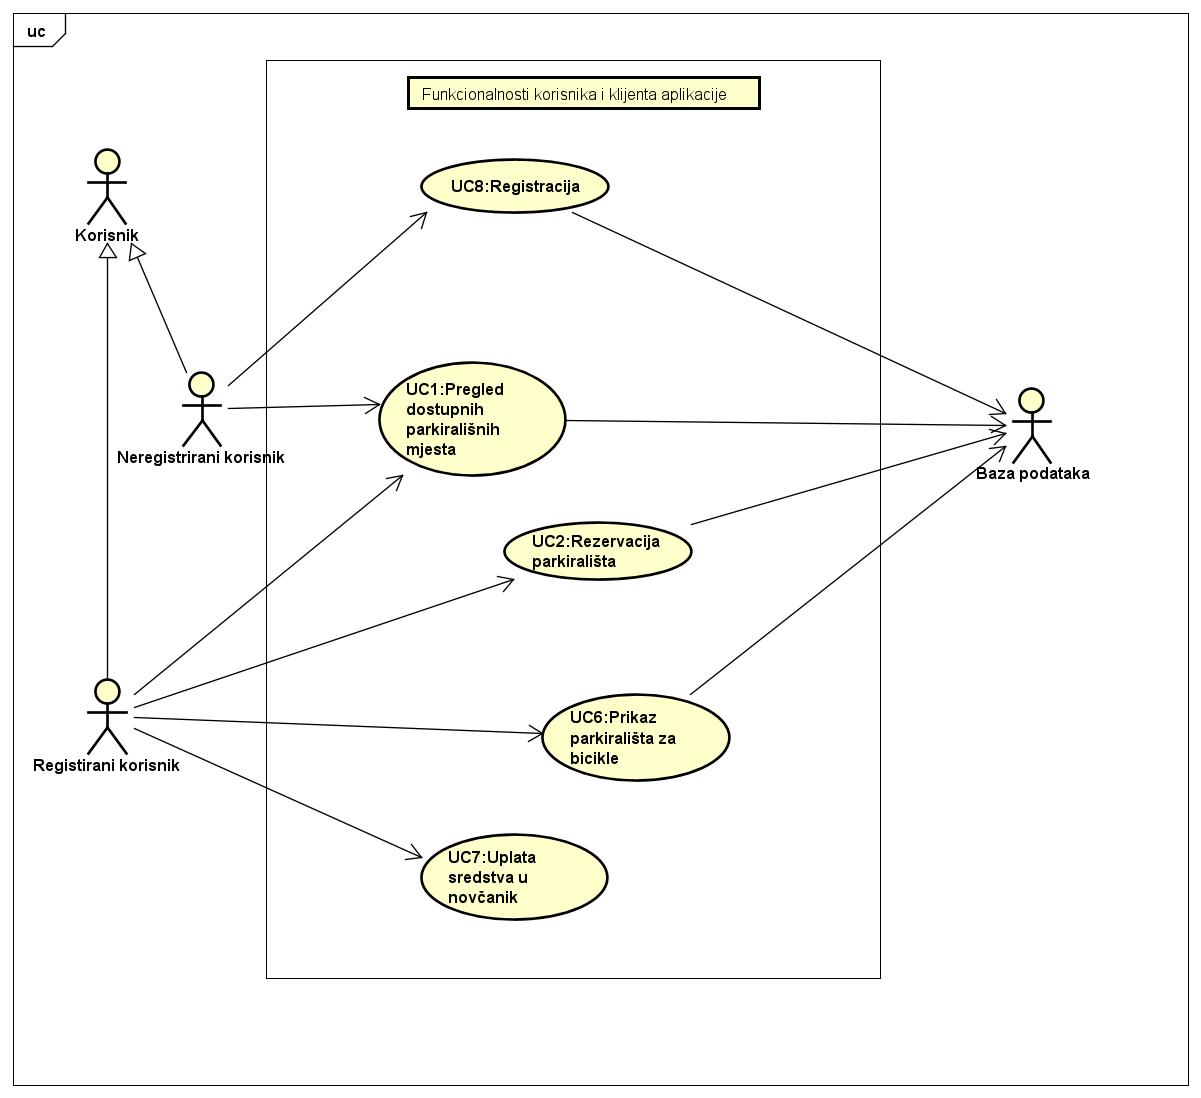
\includegraphics[width=1\linewidth,height=0.7\textheight]{../../../fer/5.semestar/progi/Projekt/dijagrami/dijagramKlijent}
	\caption{ Dijagram obrasca uporabe, funkcionalnost korisnika i klijenta}
	\label{fig:dijagramklijent}
	
\end{figure}

% TODO: \usepackage{graphicx} required
\begin{figure}
	\centering
%	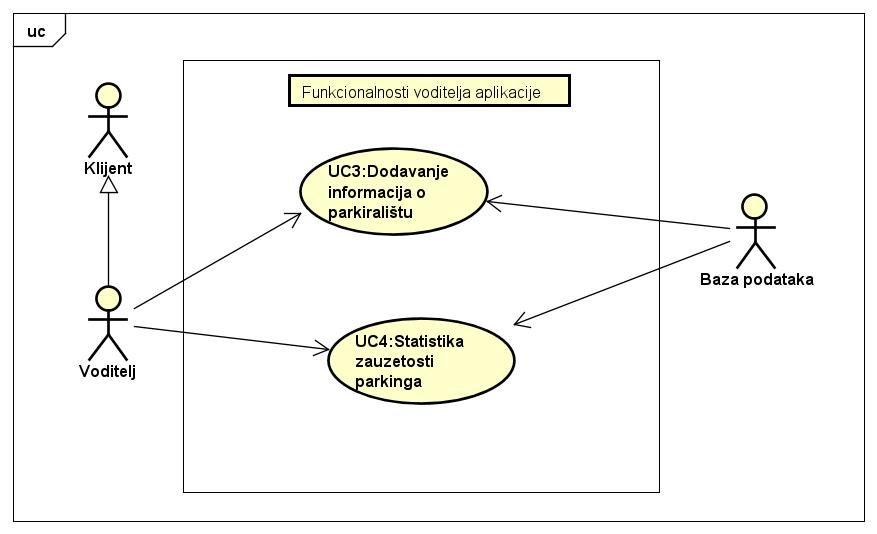
\includegraphics[width=1\linewidth]{../../../fer/5.semestar/progi/Projekt/dijagrami/dijagramVoditelj}
	\caption{Dijagram obrasca uporabe, funkcionalnost vlasnika}
	\label{fig:dijagramvoditelj}
\end{figure}

% TODO: \usepackage{graphicx} required
\begin{figure}
	\centering
%	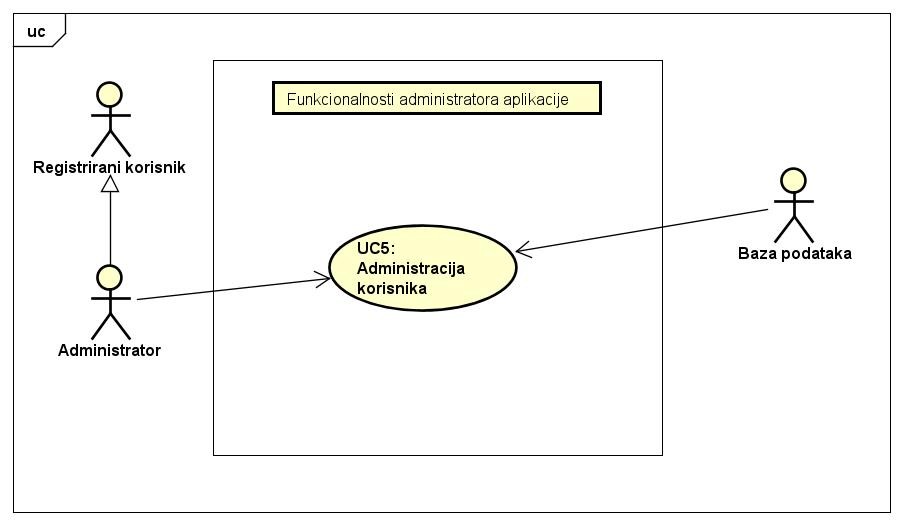
\includegraphics[width=1\linewidth]{../../../fer/5.semestar/progi/Projekt/dijagrami/dijagramAdmin}
	\caption{Dijagram obrasca uporabe, funkcionalnost administratora}
	\label{fig:dijagramadmin}
\end{figure}

\newpage
	
\subsection{Sekvencijski dijagrami}

\subsubsection{Obrazac uporabe UC1 - Pregled dostupnih parkirališta}

\textit{Klijent šalje zahtjev za prikaz kartografskog prikaza s dostupnim parkiralištima kako bi odabrao parkiralište.Aplikacija dohvaća trenutne podatke o svim parkiralištima iz baze podataka i prikazuje ih korisniku.Nakon što klijent odabere parkiralište na karti, aplikacija šalje upit bazi podataka kako bi dohvatila osnovne informacije o odabranom parkiralištu.Baza podataka odgovara na upit i šalje informacije o parkiralištu i zauzetosti parkirališnih mjesta, što aplikacija prikazuje korisniku.}

\newpage

% TODO: \usepackage{graphicx} required
\begin{figure}
	\centering
%	\includegraphics[width=1\linewidth]{"../../../fer/5.semestar/progi/Projekt/dijagrami/UC1 - Pregled dostupnih parkirališta"}
	\caption{Sekvencijski dijagram za UC1}
	\label{fig:uc1---pregled-dostupnih-parkiralista}
\end{figure}


\subsubsection{Obrazac uporabe UC2 -Rezervacija parkirališta}

\textit{Klijent šalje zahtjev za rezervaciju parkirališta odabirom parkirališta na karti i specificiranjem datuma i vremena rezervacije.Aplikacija šalje upit bazi podataka kako bi provjerila dostupnost slobodnih parkirališnih mjesta na odabranoj lokaciji za navedeni datum i vrijeme.Baza podataka provjerava dostupna mjesta i šalje informacije o slobodnim parkirališnim mjestima aplikaciji.Ako nema slobodnih mjesta na odabranom parkiralištu aplikacija obavještava klijenta o tome uz poruku.Aplikacija prikazuje klijentu dostupna slobodna mjesta i omogućuje odabir.Klijent bira slobodno parkirališno mjesto i potvrđuje rezervaciju.Aplikacija šalje upit bazi podataka za rezervaciju parkirališta.Baza podataka rezervira parkiralište i šalje potvrdu rezervacije aplikaciji.Aplikacija omogućuje klijentu plaćanje rezervacije.Aplikacija šalje potvrdu plaćanja bazi podataka.Baza podataka ažurira status rezervacije i potvrđuje plaćanje.Aplikacija šalje potvrdu rezervacije klijentu.Klijent prima potvrdu rezervacije.}


% TODO: \usepackage{graphicx} required
\begin{figure}
	\centering
%	\includegraphics[width=1\linewidth]{"../../../fer/5.semestar/progi/Projekt/dijagrami/UC2 - Rezervacija Parkirališta"}
	\caption{Sekvencijski dijagram za UC2}
	\label{fig:uc2---rezervacija-parkiralista}
\end{figure}


	

		\chapter{Arhitektura i dizajn sustava}

\subsection{Baza podataka}

\subsection{Dijagram razreda i opis razreda}


\eject
		\chapter{Implementacija i korisničko sučelje}

\section{Korištene tehnologije i alati}

\paragraph{}
{Komunikacija u timu realizirana je korištenjem aplikacije WhatsApp \footnote{\url{https://https://www.whatsapp.com/}}. Za izradu UML dijagrama korišten je alat Astah Professional\footnote{\url{https://astah.net/products/astah-professional/}}, a kao sustav za upravljanje izvornim kodom Git\footnote{\url{https://git-scm.com/}}. Udaljeni repozitorij projekta dostupan je na web platformi GitHub\footnote{\url{https://github.com/}}.
}
\paragraph{}{
Kao razvojno okruženje korišten je Microsoft Visual Studio \footnote{\url{https://visualstudio.microsoft.com/}}- integrirano je razvojno sučelje (IDE) tvrtke Microsoft. Prvenstveno se koristi za razvoj računalnih programa za operacijski sustav Windows, kao i za web-stranice, web-aplikacije, web-usluge i mobilne aplikacije. Visual Studio za razvoj softvera koristi Microsoftove platforme kao što su windows API, Windows Forms, Windows Presentation Foundation, Windows Store i Microsoft Silverlight.
}
\paragraph{}{
Aplikacija je napisana koristeći radni okvir jezik C\# \footnote{\url{https://learn.microsoft.com/en-us/dotnet/csharp/tour-of-csharp/}} za izradu backenda te React \footnote{\url{https://react.dev/}} i jezik JavaScript za izradu frontenda. React, također poznat kao React.js je biblioteka u JavaScriptu za izgradnju korisničkih sučelja. Održana je od strane Facebooka. React se najčešće koristi kao osnova u razvoju web ili mobilnih aplikacija. Složene aplikacije u Reactu obično zahtijevaju korištenje dodatnih biblioteka za interakciju s API-jem. Radni okvir Baza podataka se nalazi na poslužitelju u oblaku Microsoft Azure \footnote{\url{https://azure.microsoft.com/en-us}}.
}	



\section{Ispitivanje programskog rješenja}

\section{Dijagram razmještaja}

\paragraph{}{
UML-dijagrami razmještaja (engl. deployment diagrams) prikazuju fizičku arhitekturu programskog sustava, prikazujući razmještaj programskih artefakata na sklopovskim čvorovima ili na virtualnim okruženjima.
}

\paragraph{}{
Naš se sustav bazira na ”klijent – posluzitelj” arhitekturi, te se komunikacija između računala korisnika i poslužitelja odvija pomoću HTTP veze. Pristup web aplikaciji odvija se preko web preglednika računala korisnika. Na poslužitelju se nalaze web poslužitelj i poslužitelj baze podataka.
}

\begin{figure}[!htb]
	\centering
	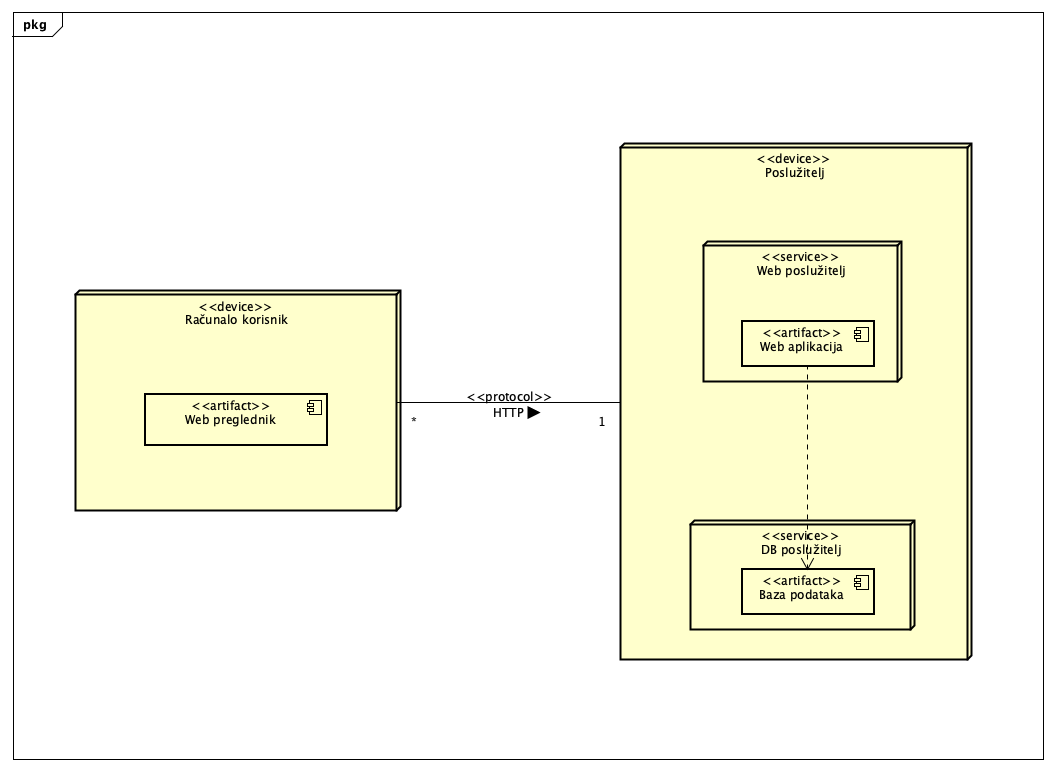
\includegraphics[width=1\linewidth]{dijagrami/DijagramRazmjestaja.png}
	\caption{Dijagram razmještaja}
	\label{fig:modelsdiagram}
\end{figure}

\section{Upute za puštanje u pogon}

\subsection{Instalacija poslužitelja baze podataka}

\paragraph{}{
	Pokretanje baze podataka radili smo unutar razvojnog okruzenja Microsoft Visual Studio. Pokretanjem debug procesa 
}




\eject
		\chapter{Zaključak i budući rad}
		\chapter*{Popis literature}
\addcontentsline{toc}{chapter}{Popis literature}

\textbf{\textit{Kontinuirano osvježavanje}}

\textit{Popisati sve reference i literaturu koja je pomogla pri ostvarivanju projekta.}


\begin{enumerate}
	
	
	\item  Programsko inženjerstvo, FER ZEMRIS, \url{http://www.fer.hr/predmet/proinz}
	
	\item  The Unified Modeling Language, \url{https://www.uml-diagrams.org/}
	
	\item  Astah Community, \url{http://astah.net/editions/uml-new}
\end{enumerate}
		\include{Literatura}
		
		\begingroup
		\renewcommand*\listfigurename{Indeks slika i dijagrama}
		%\renewcommand*\listtablename{Indeks tablica}
		%\let\clearpage\relax
		\listoffigures
		%\vspace{10mm}
		%\listoftables
		\endgroup
		\addcontentsline{toc}{chapter}{Indeks slika i dijagrama}
		
		
		
		\eject 
		
		\chapter*{Dodatak: Prikaz aktivnosti grupe}


\section{Tablica aktivnosti}



\begin{longtblr}[
	label=none,
	]{
		vlines,hlines,
		width = \textwidth,
		colspec={X[7, l]X[1, c]X[1, c]X[1, c]X[1, c]X[1, c]X[1, c]X[1, c]}, 
		vline{1} = {1}{text=\clap{}},
		hline{1} = {1}{text=\clap{}},
		rowhead = 1,
	} 
	
	\SetCell[c=1]{c}{} & \SetCell[c=1]{c}{\rotatebox{90}{\textbf{Mario Olčar}}} & \SetCell[c=1]{c}{\rotatebox{90}{\textbf{Paula Močinić}}} &	\SetCell[c=1]{c}{\rotatebox{90}{\textbf{Tomislav Marenić}}} & \SetCell[c=1]{c}{\rotatebox{90}{\textbf{Lucija Perković}}} &	\SetCell[c=1]{c}{\rotatebox{90}{\textbf{Ivan Bušljeta}}} & \SetCell[c=1]{c}{\rotatebox{90}{\textbf{Lovro De-Villa}}} &	\SetCell[c=1]{c}{\rotatebox{90}{\textbf{Matija Huđin}}} \\  
	Upravljanje projektom 		& 40 &  &  &  &  &  & \\ 
	Opis projektnog zadatka 	& 5 &  &  &  &  &  & \\ 
	
	Funkcionalni zahtjevi       &  &  &  &  & 5  &  &  \\ 
	Opis pojedinih obrazaca 	&  & 4 &  &  &  &  &  \\ 
	Dijagram obrazaca 			&  & 4 &  &  &  &  &  \\ 
	Sekvencijski dijagrami 		&  &  & 5 &  &  &  &  \\ 
	Opis ostalih zahtjeva 		& 3 &  &  &  &  &  &  \\ 
	
	Arhitektura i dizajn sustava	 &  & 15 &  &  &  &  &  \\ 
	Baza podataka				&  &  &  &  & 12 &  &   \\ 
	Dijagram razreda 			&  &  &  &  & 2 &  &   \\ 
	Dijagram stanja				&  &  &  &  &  & 2  &  \\ 
	Dijagram aktivnosti 		&  & 1 &  &  &  &  &  \\ 
	Dijagram komponenti			&  &  & 2 &  &  &  &  \\ 
	Korištene tehnologije i alati 		& 1  &  &  &  &  &  &  \\ 
	Ispitivanje programskog rješenja 	&  &  &  &  &  &  & 12 \\ 
	Dijagram razmještaja			&  &  & 2 &  &  &  &  \\ 
	Upute za puštanje u pogon 		&  &  &  &  &  &  & 1 \\  
	Dnevnik sastajanja 			& 2 &  &  &  &  &  &  \\ 
	Zaključak i budući rad 		&  & 3 &  &  &  &  &  \\  
	Popis literature 			& 1 &  &  &  &  &  &  \\  
	&  &  &  &  &  &  &  \\ \hline 
	\textit{Dodatne stavke kako ste podijelili izradu aplikacije} 			&  &  &  &  &  &  &  \\ 
	\textit{npr. izrada početne stranice} 				&  & 12 &  & 0 &  &  &  \\  
	\textit{izrada baze podataka} 		 			&  &  &  & 0  & 3 & 5 & 7\\  
	\textit{spajanje s bazom podataka} 							&  & 2 &  & 0 &  &  & 3 \\ 
	\textit{back end} 							& 4 &  &  &  & 4 & 7 & 8 \\  
	&  &  &  &  &  &  &\\ 
\end{longtblr}

\eject
		
		
	\end{document} %naredbe i tekst nakon ove naredbe ne ulaze u izgrađen dokument 
	
	
